\chapter{Code-Based Cryptography}
\subsection*{Public-Key Encryption}
\begin{itemize}
    \item \textbf{Goal}: Confidentiality, when communicating over an
          insecure channel.
    \item \textbf{Main feature}: The two communicating parties
          do not share any secrets. They only share
          \emph{public information} that has been \emph{authenticated}.
\end{itemize}
\begin{figure}[!htbp]
    \centering
    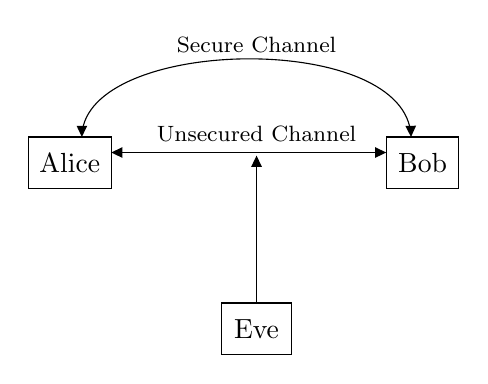
\begin{tikzpicture}[x=0.75pt,y=0.75pt,yscale=-1,xscale=1]
        % Text Node
        \draw    (118.26,145.79) -- (158.26,145.79) -- (158.26,170.79) -- (118.26,170.79) -- cycle  ;
        \draw (138.26,158.29) node   [align=left] {Alice};
        % Text Node
        \draw    (290.76,145.79) -- (325.76,145.79) -- (325.76,170.79) -- (290.76,170.79) -- cycle  ;
        \draw (308.26,158.29) node   [align=left] {Bob};
        % Text Node
        \draw    (211.26,225.79) -- (245.26,225.79) -- (245.26,250.79) -- (211.26,250.79) -- cycle  ;
        \draw (228.26,238.29) node   [align=left] {Eve};
        % Text Node
        \draw (228.26,144.29) node  [font=\footnotesize] [align=left] {Unsecured Channel};
        % Text Node
        \draw (228.26,101.29) node  [font=\footnotesize] [align=left] {Secure Channel};
        % Connection
        \draw    (161.26,153.29) -- (287.76,153.29) ;
        \draw [shift={(290.76,153.29)}, rotate = 180] [fill={rgb, 255:red, 0; green, 0; blue, 0 }  ][line width=0.08]  [draw opacity=0] (5.36,-2.57) -- (0,0) -- (5.36,2.57) -- cycle    ;
        \draw [shift={(158.26,153.29)}, rotate = 0] [fill={rgb, 255:red, 0; green, 0; blue, 0 }  ][line width=0.08]  [draw opacity=0] (5.36,-2.57) -- (0,0) -- (5.36,2.57) -- cycle    ;
        % Connection
        \draw    (228.26,225.79) -- (228.26,157.79) ;
        \draw [shift={(228.26,154.79)}, rotate = 450] [fill={rgb, 255:red, 0; green, 0; blue, 0 }  ][line width=0.08]  [draw opacity=0] (5.36,-2.57) -- (0,0) -- (5.36,2.57) -- cycle    ;
        % Connection
        \draw    (144.4,142.22) .. controls (152.1,97.9) and (295.61,95.5) .. (302.43,142.83) ;
        \draw [shift={(302.68,145.79)}, rotate = 268.7] [fill={rgb, 255:red, 0; green, 0; blue, 0 }  ][line width=0.08]  [draw opacity=0] (5.36,-2.57) -- (0,0) -- (5.36,2.57) -- cycle    ;
        \draw [shift={(144.08,145.79)}, rotate = 270.5] [fill={rgb, 255:red, 0; green, 0; blue, 0 }  ][line width=0.08]  [draw opacity=0] (5.36,-2.57) -- (0,0) -- (5.36,2.57) -- cycle    ;
    \end{tikzpicture}
\end{figure}
\subsection*{Basic RSA Encryption Scheme}
\subsubsection*{Key Generation}
Alice does the following:
\begin{enumerate}
    \item Randomly select two large prime numbers, $ p $ and $ q $.
    \item Compute $ n=pq $ and $ \phi(n)=(p-1)(q-1) $.
    \item Select arbitrary $ e $, $ 1<e<\phi(n) $ with $ \gcd\bigl(e,\phi(n)\bigr)=1 $.
    \item Compute $ d= e^{-1}\mod \phi(n) $.
    \item Alice's public key is $ (n,e) $, while her private key is $ d $.
          The only known way to recover $ d $ from the public key is to first factor
          $ n $ to find $ p $ and $ q $. So, the private key remains secret
          to Alice as long is $ n $ is large enough so that no one else can factor it.
\end{enumerate}
\subsubsection*{Encryption}
To encrypt a message for Alice, Bob does:
\begin{enumerate}
    \item Obtain an authentic copy of Alice's public key $ (n,e) $.
    \item Represent the message $ m $ as an integer $ [0,n-1] $.
    \item Compute $ c= m^e \mod n $.
    \item Send $ c $ to Alice over the unsecured channel.
\end{enumerate}
\subsubsection*{Decryption}
To decrypt $ c $, Alice does:
\begin{enumerate}
    \item Compute $ m= c^d\mod n $.
\end{enumerate}
\subsection*{The Threat of Quantum Computers}
\begin{itemize}
    \item The security of RSA is based on the hardness of factoring $ n $.
    \item It has been known since 1994 that factoring $ n $ is easy
          on a \emph{quantum computer}.
    \item \emph{Elliptic-curve cryptography}, a widely used alternative to
          RSA can also be broken easily by quantum computers.
    \item We are still \emph{very far away} from being able to build
          large-scale quantum computers.
    \item Nonetheless, it seems prudent to develop public-key encryption
          schemes that \emph{resist attacks even by quantum computers}.
\end{itemize}
\subsection*{McEliece Public-Key Encryption Scheme (1978)}
\begin{itemize}
    \item \textbf{Security} is based on the fact that decoding
          a random (binary) linear code is \emph{NP-hard}.
    \item \textbf{Idea}:
          \begin{itemize}
              \item Select a code $ C $ for which an efficient decoding algorithm is known.
              \item Disguise $ C $ to get ``random looking'' code $ \hat{C} $.
              \item $ \hat{C} $ is your \emph{public key}, while the ``disguising factor''
                    is your \emph{private key}.
              \item \textbf{Encryption}: Encode $ \symbf{m} $ to get
                    $ \hat{\symbf{c}}\in\hat{C} $, add a random error $ \symbf{e} $ to
                    $ \hat{\symbf{c}} $ to get $ \hat{\symbf{r}} $ ($ \hat{\symbf{r}}=\hat{\symbf{c}}+\symbf{\symbf{e}} $),
                    and send $ \hat{\symbf{r}} $.
              \item \textbf{Decryption}: Use the ``disguising factor'' to
                    convert the decoding problem to one for $ C $ ($ \symbf{r}=\symbf{c}+\symbf{e} $), and
                    then use the decoding algorithm for $ C $ to recover $ \symbf{e} $ and $ \symbf{m} $.
          \end{itemize}
\end{itemize}
\subsubsection*{Key Generation}
Alice does the following:
\begin{enumerate}
    \item Select a $ k\times n $ generator matrix $ G $ for a $ t $-error
          correcting \textbf{binary Goppa code} $ C $.
    \item Select a random $ k\times k $ binary invertible matrix $ S $.
    \item Select a random $ n\times n $ permutation matrix $ P $.
    \item Compute $ \hat{G}=SGP $ ($ \hat{G} $ is a $ k\times n $ matrix of rank $ k $).
    \item Alice's \emph{public key} is $ (\hat{G},t) $, while her \emph{private key}
          is $ (G,S,P) $.
\end{enumerate}
\fbox{\textbf{Conjecture}: $ \hat{G} $ is indistinguishable from a random
    $ k\times n $ binary matrix of rank $ k $.}
\subsubsection*{Encryption}
To encrypt a message for Alice, Bob does:
\begin{enumerate}
    \item Obtain an authentic copy of Alice's public key $ (\hat{G},t) $.
    \item Represent the message as a binary vector $ \symbf{m} $ of length $ k $.
    \item Select a random binary vector $ \symbf{e}\in V_n(\mathbf{Z}_2) $
          of weight $ t $.
    \item Compute $ \hat{\symbf{r}}=\symbf{m}\hat{G}+\symbf{e} $,
          and send $ \hat{\symbf{r}} $ to Alice.
\end{enumerate}
\subsubsection*{Decryption}
To decrypt $ \hat{\symbf{r}} $, Alice does the following:
\begin{enumerate}
    \item Compute $ \symbf{r}=\hat{\symbf{r}}P^{-1} $.

          [Note: $ \symbf{r}=\hat{\symbf{r}}P^{-1}=\symbf{m}\hat{G}P^{-1}+\symbf{e}P^{-1}
              =(\symbf{m}SGP)P^{-1}+\symbf{e}P^{-1}=(\symbf{m}S)G+\symbf{e}P^{-1} $]
    \item Use the decoding algorithm for $ C $ to recover $ \symbf{m}^\prime =\symbf{m}S $.
    \item Compute $ \symbf{m}=\symbf{m}^\prime S^{-1} $.
\end{enumerate}
\textbf{Security} is based on the hardness of decoding $ \hat{C} $
(the code generated by $ \hat{G} $).
\subsection*{Implementation Notes}
\begin{itemize}
    \item \textbf{Suggested parameters}: $ n=4096 $, $ k=3496 $, and $ t=50 $.
    \item Encryption is very fast.
    \item Decryption is relatively fast.
    \item Appears to resist quantum attacks.
\end{itemize}
\subsubsection*{Using Other Codes}
Proposals that replace the Goppa codes with RS codes, LDPC codes,
convolutional codes, etc., have all been broken.

One secure alternative is to use ``\emph{quasi-cyclic MDPC codes}.''
